\chapter{State of the Art}

\section{The context}

    \subsection{The ARCOS Project}
    \textbf{ARCOS} (ARCtic Observatory for Copernicus SEA Security Service) is an EU-funded project (specifically from the \textit{European Union’s Horizon 2020 research and innovation programme}) whose goal is to design and implement an early warning system that provides continuous monitoring of the \textbf{Arctic region} \cite{arcos}. 
    
    Designed to create actionable security products by processing and merging multi-sensor data, the ARCOS system integrates information available space, non-space sources and products available from Copernicus Services \cite{copernicus}. 
    
    The project system ARCOS handle information at three different levels of scale and user interaction:
    
    \begin{enumerate}
    \item \textbf{Automatic early-warning system}: Integration of multi-channel data sources with the goal of triggering alerts in the region when certain conditions are met. Automatic early warnings are generated when anomalous behaviours are detected, such as the discovery of suspicious targets or large-scale exploitation of natural resources.
    
    \item \textbf{User Driven Alert System} by providing user guidance on the specific location and type of observation objects desired, alarms can be configured based on more specific information, such as activity patterns.
    
    \item \textbf{Geospatial Intelligence Products}. Thanks to the warnings previously generated, geospatial intelligence products requiring human intervention are provided at the user's request. These products require extensive contextual analysis, typically requiring coordinated action at more than one location.
    \end{enumerate}
    
    \begin{figure}[H]
        \centering
        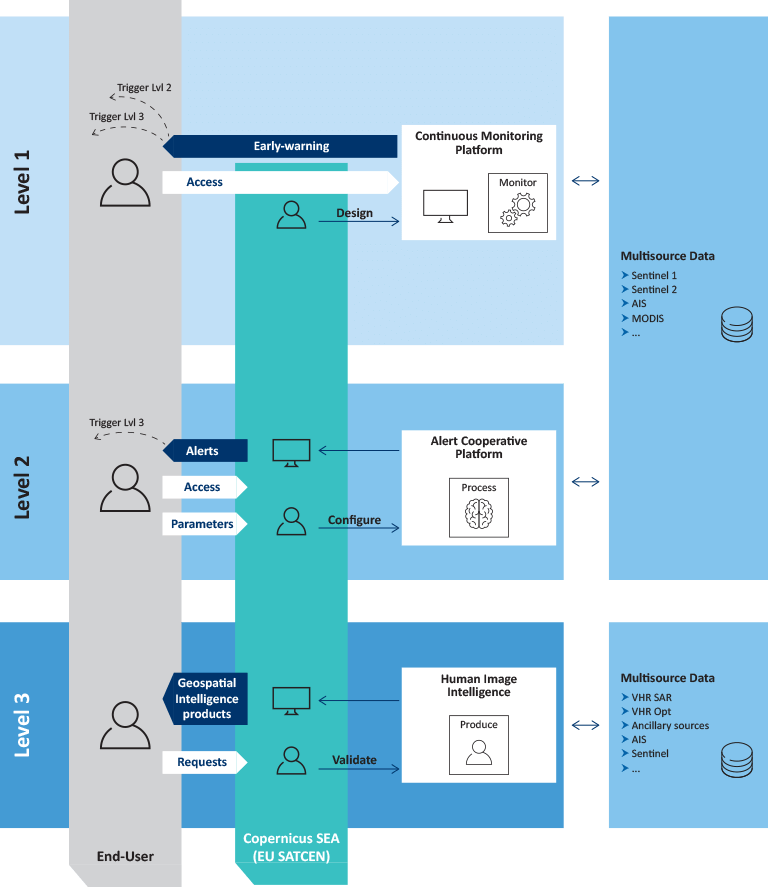
\includegraphics[width=13cm]{Images/1/arcos-design.png}
        \caption{ARCOS Project platform design \cite{arcos}}
    \end{figure}
        

    
\newpage
\section{The AIS Data}
    \subsection{Introduction}
    The \textit{\textbf{Automatic Identification System}} (AIS) is an automatic tracking system widely used by \textit{Vessel Traffic Services} (VTS). AIS is crucial in order to grant safety and security in maritime operations.
    It bases its operation on a transceiver on ships that sends data to others receivers or to satellites.
    
    AIS information includes a variety of data regarding the real-time status of a ship during a voyage, e.g. its unique identifier, position, ship status, and speed. This information is very useful when displayed on the screen of a \textit{Electronic Chart Display and Information System} (ECDIS).
    
    The \textit{International Maritime Organization} (IMO) requires AIS system to be installed on board ships of 300 gross tonnage (i.e. a nonlinear measure of a ship's overall internal volume) or more, cargo ships of 500 gross tonnage and all passenger ships, regardless of size \cite{ais_regulations}.
    
    According to the current regulations AIS systems should:
    \begin{itemize}
        \item Automatically relay information - including vessel identity, type, position, course, speed, navigational status, and other safety-related information
        \item Automatically receive such information from similarly equipped vessels; 
        \item Monitor and track ships;
        \item Exchange data with coast facilities.
    \end{itemize}

    Despite the strict regulations in place on AIS systems, for a variety of reasons, ships may turn off their AIS transceivers or, much more frequently, technical errors may occur that affect the continuity of the reception of AIS messages.
    
    \subsection{A focus on Satellite AIS}
    AIS is designed to assist a ship's watch-keeping officers and to enable maritime authorities to track and monitor ship movements. AIS integrates a standardized VHF (Very High Frequency) transceiver with a positioning system, with other electronic navigation sensors, such as a gyrocompass or rate-of-turn indicator. Vessels equipped with AIS transceivers can be tracked by AIS base stations along coastlines or, when out of range of terrestrial networks, via a high number of satellites equipped with specialized AIS receivers. 
    \\
    Satellite Automatic Identification System (\textbf{S-AIS}) is based on satellite infrastructure and in particular on satellites in Low Earth Orbit (LEO). These satellites are equipped with AIS receivers and the received messages are retransmitted in a broadcast system.
    The just described technical solution increases the range of AIS and makes it possible to cover an area between 2\% and 4\% of the Earth's surface with a LEO satellite. \cite{dbscan_ais}.
    
    The main problem posed by S-AIS is the collision of data packets: If a large number of ships use the same transmission time slot, the satellite component receiving the AIS messages might have problems correctly identifying the packet affiliation.
    \\
    The main reason for this is that S-AIS operates in a larger area covering a wide area, and therefore collects signals from multiple transmitters, resulting in collisions of data packets.
    As a result, data belonging to different packets get mixed and it is not possible to recover the packet in its original form. As a result, important parts of messages from AIS are lost, so a considerable number of messages are not recognised and forwarded to a terrestrial part of the system. As a result, it is not possible to monitor part of the trajectory of ships \cite{dbscan_ais}.
    
    % https://en.wikipedia.org/wiki/Automatic_identification_system#cite_note-1:~:text=External%20links-,Viewing%20and%20using%20AIS%20data,-%5Bedit%5D
    
    
\clearpage  

\section{Anomaly Detection Techniques}

    \textbf{Anomaly detection} is a branch in data mining that identifies event or observations that deviate from the normal behavior of a data set \cite{anomaly_detection}. Anomaly detection is applicable in a very large number and variety of domains and that makes it so widely used.
    \\
    Anomalous data can indicate critical incidents, such as a technical malfunction, or potential opportunities, such as changing consumer behavior. Machine learning techniques are increasingly being used to automate anomaly detection.
    
    \subsection{Time Series}
    The starting point for a well-functioning anomaly detection algorithm is the analysis of time series.
    \\
    Time series are sequences of values over time. This means that each entry in the data set can be viewed as a pair of two elements: a timestamp for when the metric was measured, and the set of values associated with that metric at that time. 
    \\ 
    Time series data should not be viewed as a projection of the data set; rather, it contains the information necessary to make fairly accurate guesses about what to expect in the future. Anomaly detection systems use these expectations to identify actionable signals in your data and detect outliers that indicate certain relevant events in your business.
    
    \subsubsection{Time Series in Maritime field}
    In the maritime application domain of anomaly detection, the just mentioned time series are sequences of AIS messages containing the whole set of various parameters representing the state of the ship, i.e. real-time information collected on board a ship by numerous sensors (such as GPS locator, accelerometer, gyroscope, etc.). 
    In S-AIS (Satellite AIS) data, messages are sent to satellites at an average frequency of thirty seconds, but this can be varied depending on ship speed or base station instructions. 
    \\
    The described time series represent the trajectories of the ships, each of them could be defined as a finite sequence of positions of the ship received in chronological order. The problem of packet collisions mentioned leads to a lack of data in the sequence. Thus, such a data point corresponds to a multi-dimensional feature vector of the moving ship at a particular time, and the packet collision problem introduces noise or lack of data.

    \subsection{Clustering Techniques Overview}
    In the field of data analysis, the general task of dividing data points into groups such that the data points in the same groups are more similar to other data points in the same group than those in other groups is called \textbf{clustering} \cite{clustering}.
    \\
    As first important classification, clustering is defined:
    
    \begin{itemize}
    \item \textbf{Hard Clustering} when each data point either belongs entirely to a cluster or does not.
    \item \textbf{Soft Clustering} each data point is not placed in a separate cluster, but is assigned a probability of being included in those clusters.
    \end{itemize}
    \\
    
    \begin{figure}[H]
        \centering
        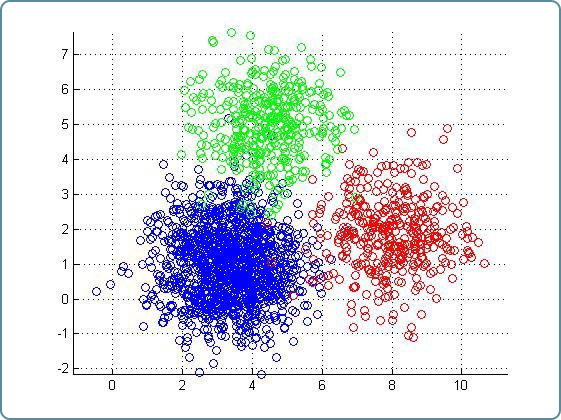
\includegraphics[width=9cm]{Images/1/clustering.png}
        \caption{Visualization of hard clustering technique}
    \end{figure}
        
    
    A basic example of a clustering model is \textbf{K-means}. It comes from the family of \textit{Centroid models} and aims to iteratively partition n data points into k clusters in which each observation belongs to the cluster with the closest mean.
    Its clustering process can be summarized in 5 points:
    
    \begin{enumerate}
        \item Specify the desired number of clusters K;
        \item Randomly assign each data point to a cluster;
        \item Calculate the centres for each cluster;
        \item Re-assign each point to the nearest cluster centre;
        \item Recalculate the cluster centroids;
        \item Repeat steps 4 and 5 until no more improvements are possible.
    \end{enumerate}
    
    \begin{figure}[H]
        \centering
        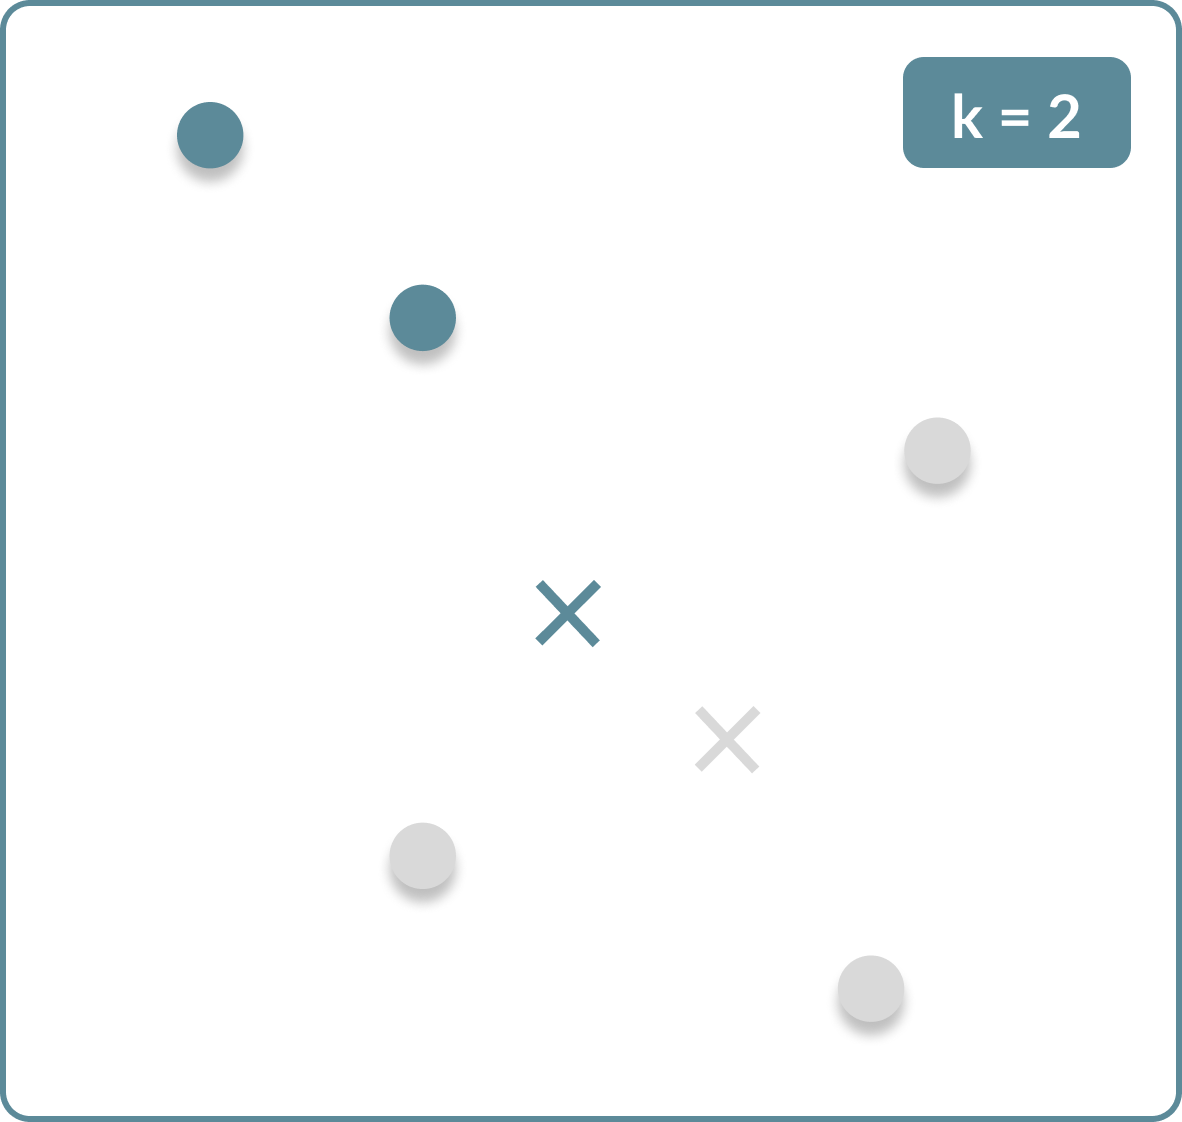
\includegraphics[width=9cm]{Images/1/kmeans.png}
        \caption{Data points and centroids in k-means clustering}
    \end{figure}
    
    There are more than 100 known clustering algorithms, and each method follows a different set of rules for defining similarity between data points. But the class of clustering algorithms that is highlighted in this work is \textbf{density-based clustering algorithms}. These models search the data space for regions of varying density of data points in the data space. It isolates different regions of varying density and assigns the data points within those regions to the same cluster. Popular examples of density models include DBSCAN and OPTICS.
    
    
    \subsection{DBSCAN}
    \textbf{Density-based spatial clustering of Applications with Noise} (DBSCAN) is an algorithm for clustering data based on density.
    \\
    The algorithm works with a given set of points in a given space, it groups the points that are close enough to each other and labels the points that are in low-density regions alone as outliers. DBSCAN is one of the most common clustering algorithms and is also one of the most cited in the scientific literature.
    \\
    In order to represent data points in a space, the concept of dimension must be defined. Namely, for each data point, the characteristics - necessarily numerical - must be defined, which then form the coordinates in the space where the density analysis is performed. It is very important to accurately select the numerical features of the data set, based on the ones we want to highlight in order to get back similarities or differences with this algorithm.
    \\
    Considering a set of points in a space to be clustered. Let $\varepsilon$ be a parameter that specifies the radius of a neighborhood with respect to a point.
    For the purposes of the DBSCAN clustering, the points are divided into \textbf{core points}, \textbf{reachable points}, and \textbf{outliers} as follows:
        
    \begin{itemize}
    \item A point \textit{p} is a core point if at least \textit{minPts} points are within distance $\varepsilon$ of it.
    \item A point \textit{q} is directly reachable from \textit{p} if point \textit{q} is within distance $\varepsilon$ from core point \textit{p}. Points are considered directly reachable only from core points.
    \item A point \textit{q} is reachable from \textit{p} if there is a path \textit{$p_1$}, ..., \textit{$p_n$} with \textit{$p_1$} = \textit{p} and \textit{$p_n$} = \textit{q}, where every \textit{$p_{i+1}$} is directly reachable from \textit{$p_i$}. Note that this implies that the starting point and all points on the path must be core points, with the possible exception of \textit{q}.
    \item All points that are not reachable from any other point are \textbf{outliers} or \textbf{noise points}.
    \end{itemize}
    
    % https://www.youtube.com/watch?v=4b5d3muPQmA
    
    \subsubsection{A pratical implementation example}
    